\chapter{Systemarchitektur des Quadrocopters}
\label{chap:Systemarchitektur}
Zu Beginn wird in diesem Kapitel die Hardwarearchitektur sowie die Kommunikationsstruktur vorgestellt. Ziel ist es einen �berblick der verbauten Sensoren und Recheneinheiten sowie deren Vernetzung untereinander zu erlangen. 
\section{Hardwareaufbau}
\label{sec:Hardwareaufbau}
Zum Einsatz kommt der AscTec Pelican der Firma ASCENDING TECHNOLOGIES. Dieser Quadrocopter ist speziell f�r die Forschung entworfen worden. Seine Turmstruktur erm�glicht eine einfache Integration zus�tzlicher Sensoren und Nutzlasten. Durch diese Flexibilit�t im Aufbau ist es Ziel dieses Teilkapitels einen �berblick zu geben, wo die einzelnen Komponenten positioniert sind. Begleitend zum Text ist der Aufbau in Abbildung \ref{fig:hardwareaufbau} sowie etwas ausf�hrlicher, mit den Daten der Komponenten, im Anhang dargestellt.


F�r jeder der vier mit einem Propellor verbundenen Elektromotoren, ist ein separate Motorcontroller zust�ndig. Diese sorgen daf�r, dass sich die von der \gls{FCU} angeforderten Drehzahlen einstellt. Die FCU ist die zentrale Steuer- und Regeleinheit des Quadrocopters. Zus�tzlich ist auf ihr die Inertialsensorik integriert. Diese besteht aus einem Beschleunigungssensor, einem Lagesensor sowie einem Drucksensor zur Messung der Flugh�he. Ein Drucksensor ist zur H�henbestimmung in geschlossenen R�umen nicht eignet, da erst ab einer H�he von 5m zuverl�ssige Werte liefert. Deshalb wurde in einer vorangegangen Arbeit die Hardware (lITERAURVERWIES JAN) um ein Modul zur Messung der H�he im Indoorbereich erweitert. Auf diesem Modul befinden sich ein zwei Infarotsensoren f�r den Nahbereich (HIER MUSS NOCH DIE RANGE EINGETRAGEN WERDEN JAN) und einem Ultrashallsenor f�r Entfernungen von bis zu 5 m. Da f�r diese Arbeit die Navigation in der horizontale Ebene den Schwerpunkt darstellt, wird dieses Modul nicht weiter behandelt.


Um in der horizontalen navigieren zu k�nnen muss, die Position in der x-y Ebene (VGL kOORDINATENSYSTEME) bekannt sein. Damit diese bestimmt werden kann wurde in die Turmstruktur ein Lasersanner der Firma Hokuyo integriert.

Damit zur Berechnung der Position sowie Implementierung weiterer Algorithmen und Funktionen ausreichend Rechenleistung vorhanden ist, wurde der Quadrocopter mit einem zus�tzlichen Odroid-X Mikrocomputer ausgestattet.


Nun sollte man einen �berblick �ber die im Quadrocopter verbauten Komponenten besitzen. Darauf wie diese Einheiten untereinander vernetzt sind, wird im folgenden Kapitel \ref{sec:Kommunikationsarchitekur} eingegangen.

     

%In der Grundausstattung enthalten ist das AutoPilot Board auch \gls{FCU}  genannt. Diese Board ist die Steuer- und Regeleinheit des \gls{UAV}, zu deutsch \glqq unbemanntes Luftfahrzeug \grqq. Die Inertialsensorik befindet sich ebenfalls auf dieser Platine. Diese beinhaltet einen Beschleunigungssensor, einen Lagesensor sowie einen Drucksensor zur H�henbestimmung.



 %Wie sich aus dem Name schlie�en l�sst ist diese Einheit zur Steuerung und Regelung des \gls{UAV}, zu deutsch unbemanntes Luftfahrzeug. 
%Darauf integriert sind die Inertialsensoren wie Beschleunigungssensor, Lagesensor(Gyro), Kompass und Drucksensor. 


\begin{figure}
	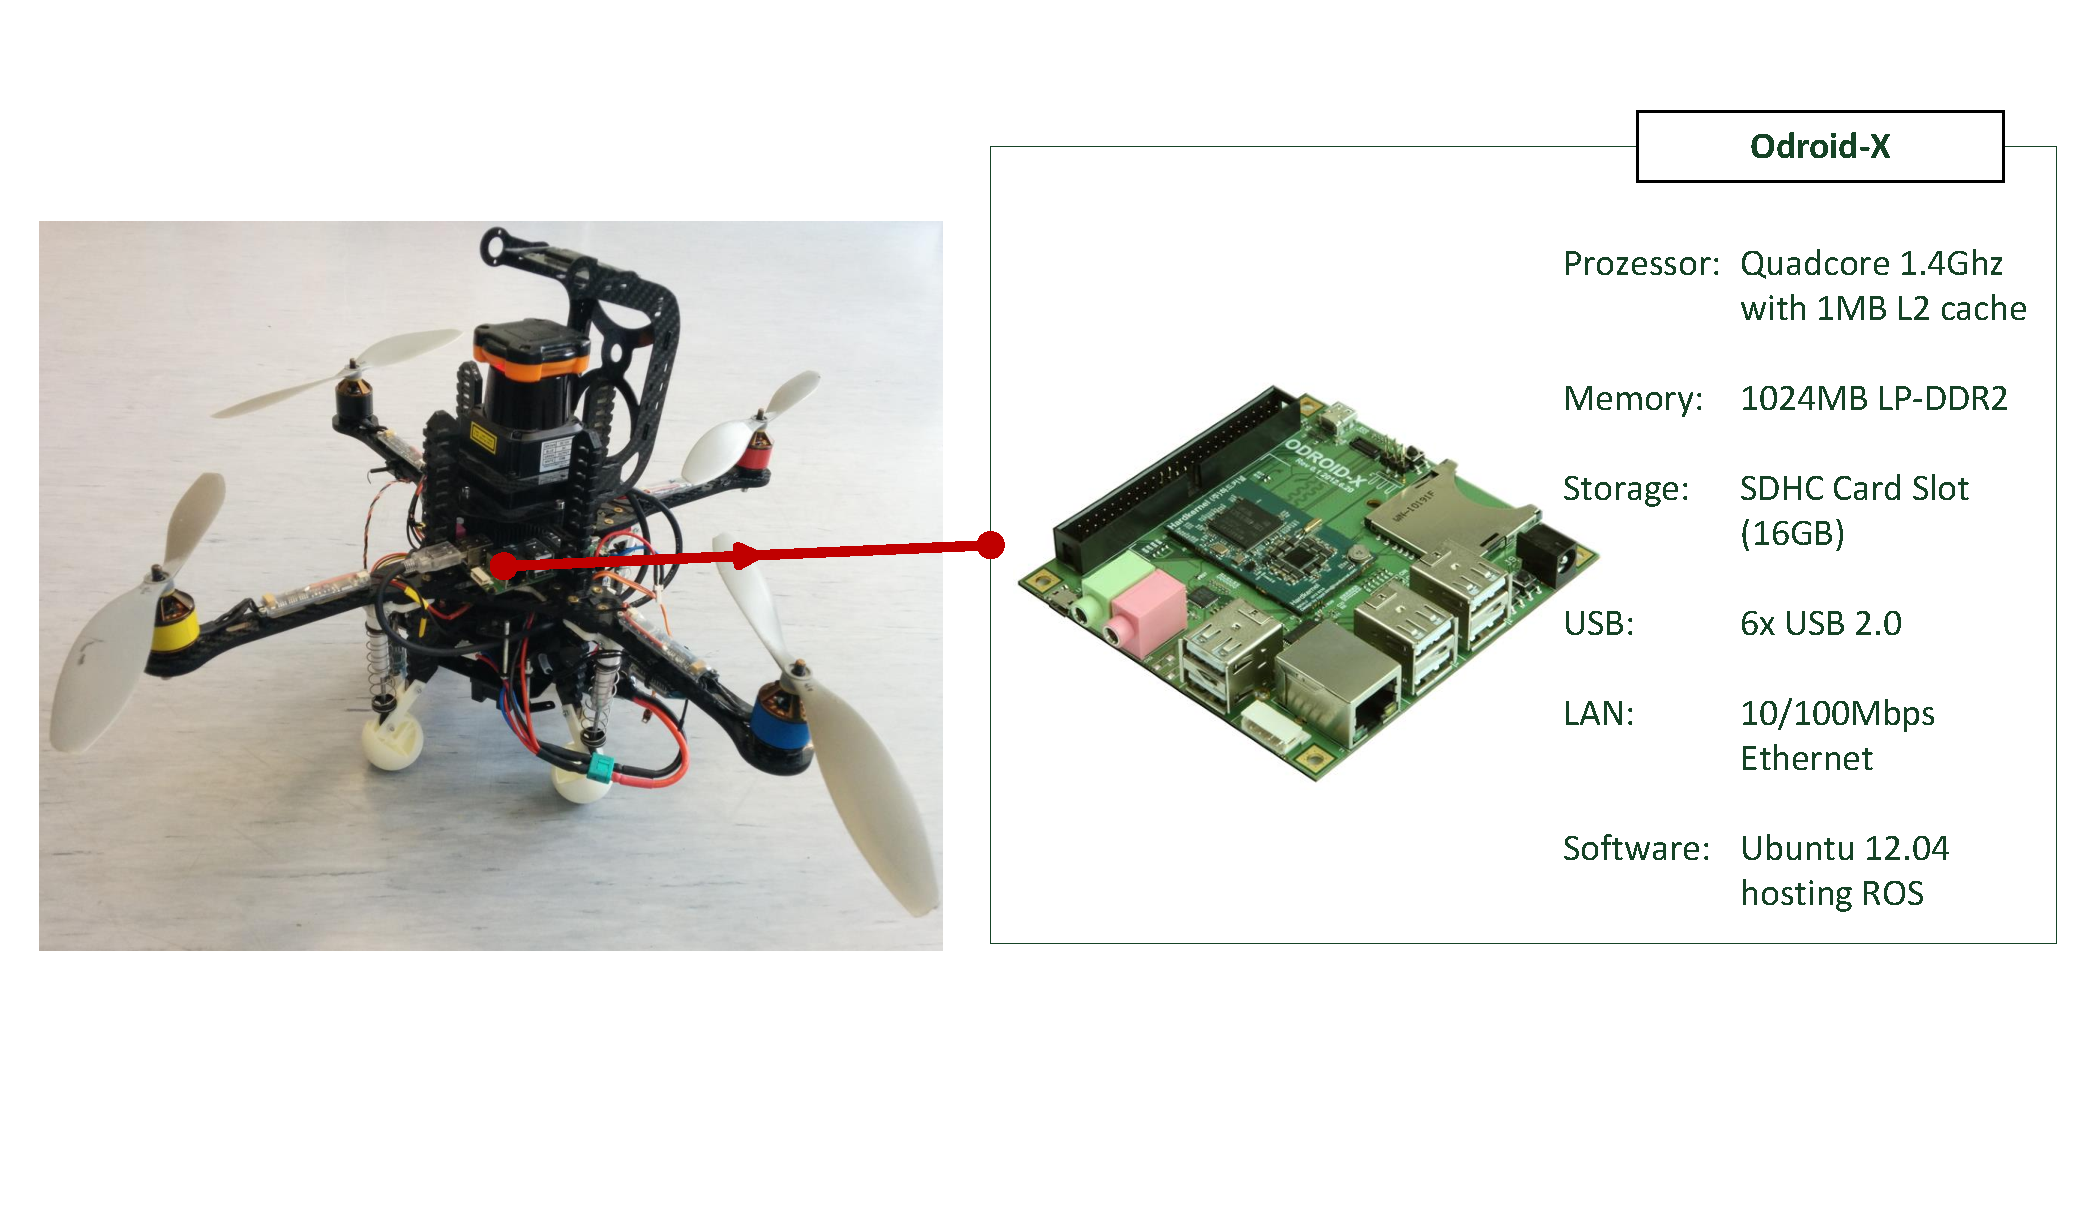
\includegraphics[width = 0.75\textwidth]{images/quad_odroid}
	\caption[Hardwareaufbau]{Hardwareaufbau des Quadrocopters...DIESE GRAFIK IST EIN PLATZHALTER GRAFIK NUR MIT NAMEN DER KOMPONENTEN}
	\label{fig:hardwareaufbau}
\end{figure}

\section{Kommunikationsstruktur}
\label{sec:Kommunikationsarchitekur}

Die Kommunikationsstruktur wird in Abbildung \ref{fig:Kommunikationsstruktur}
\begin{figure}
	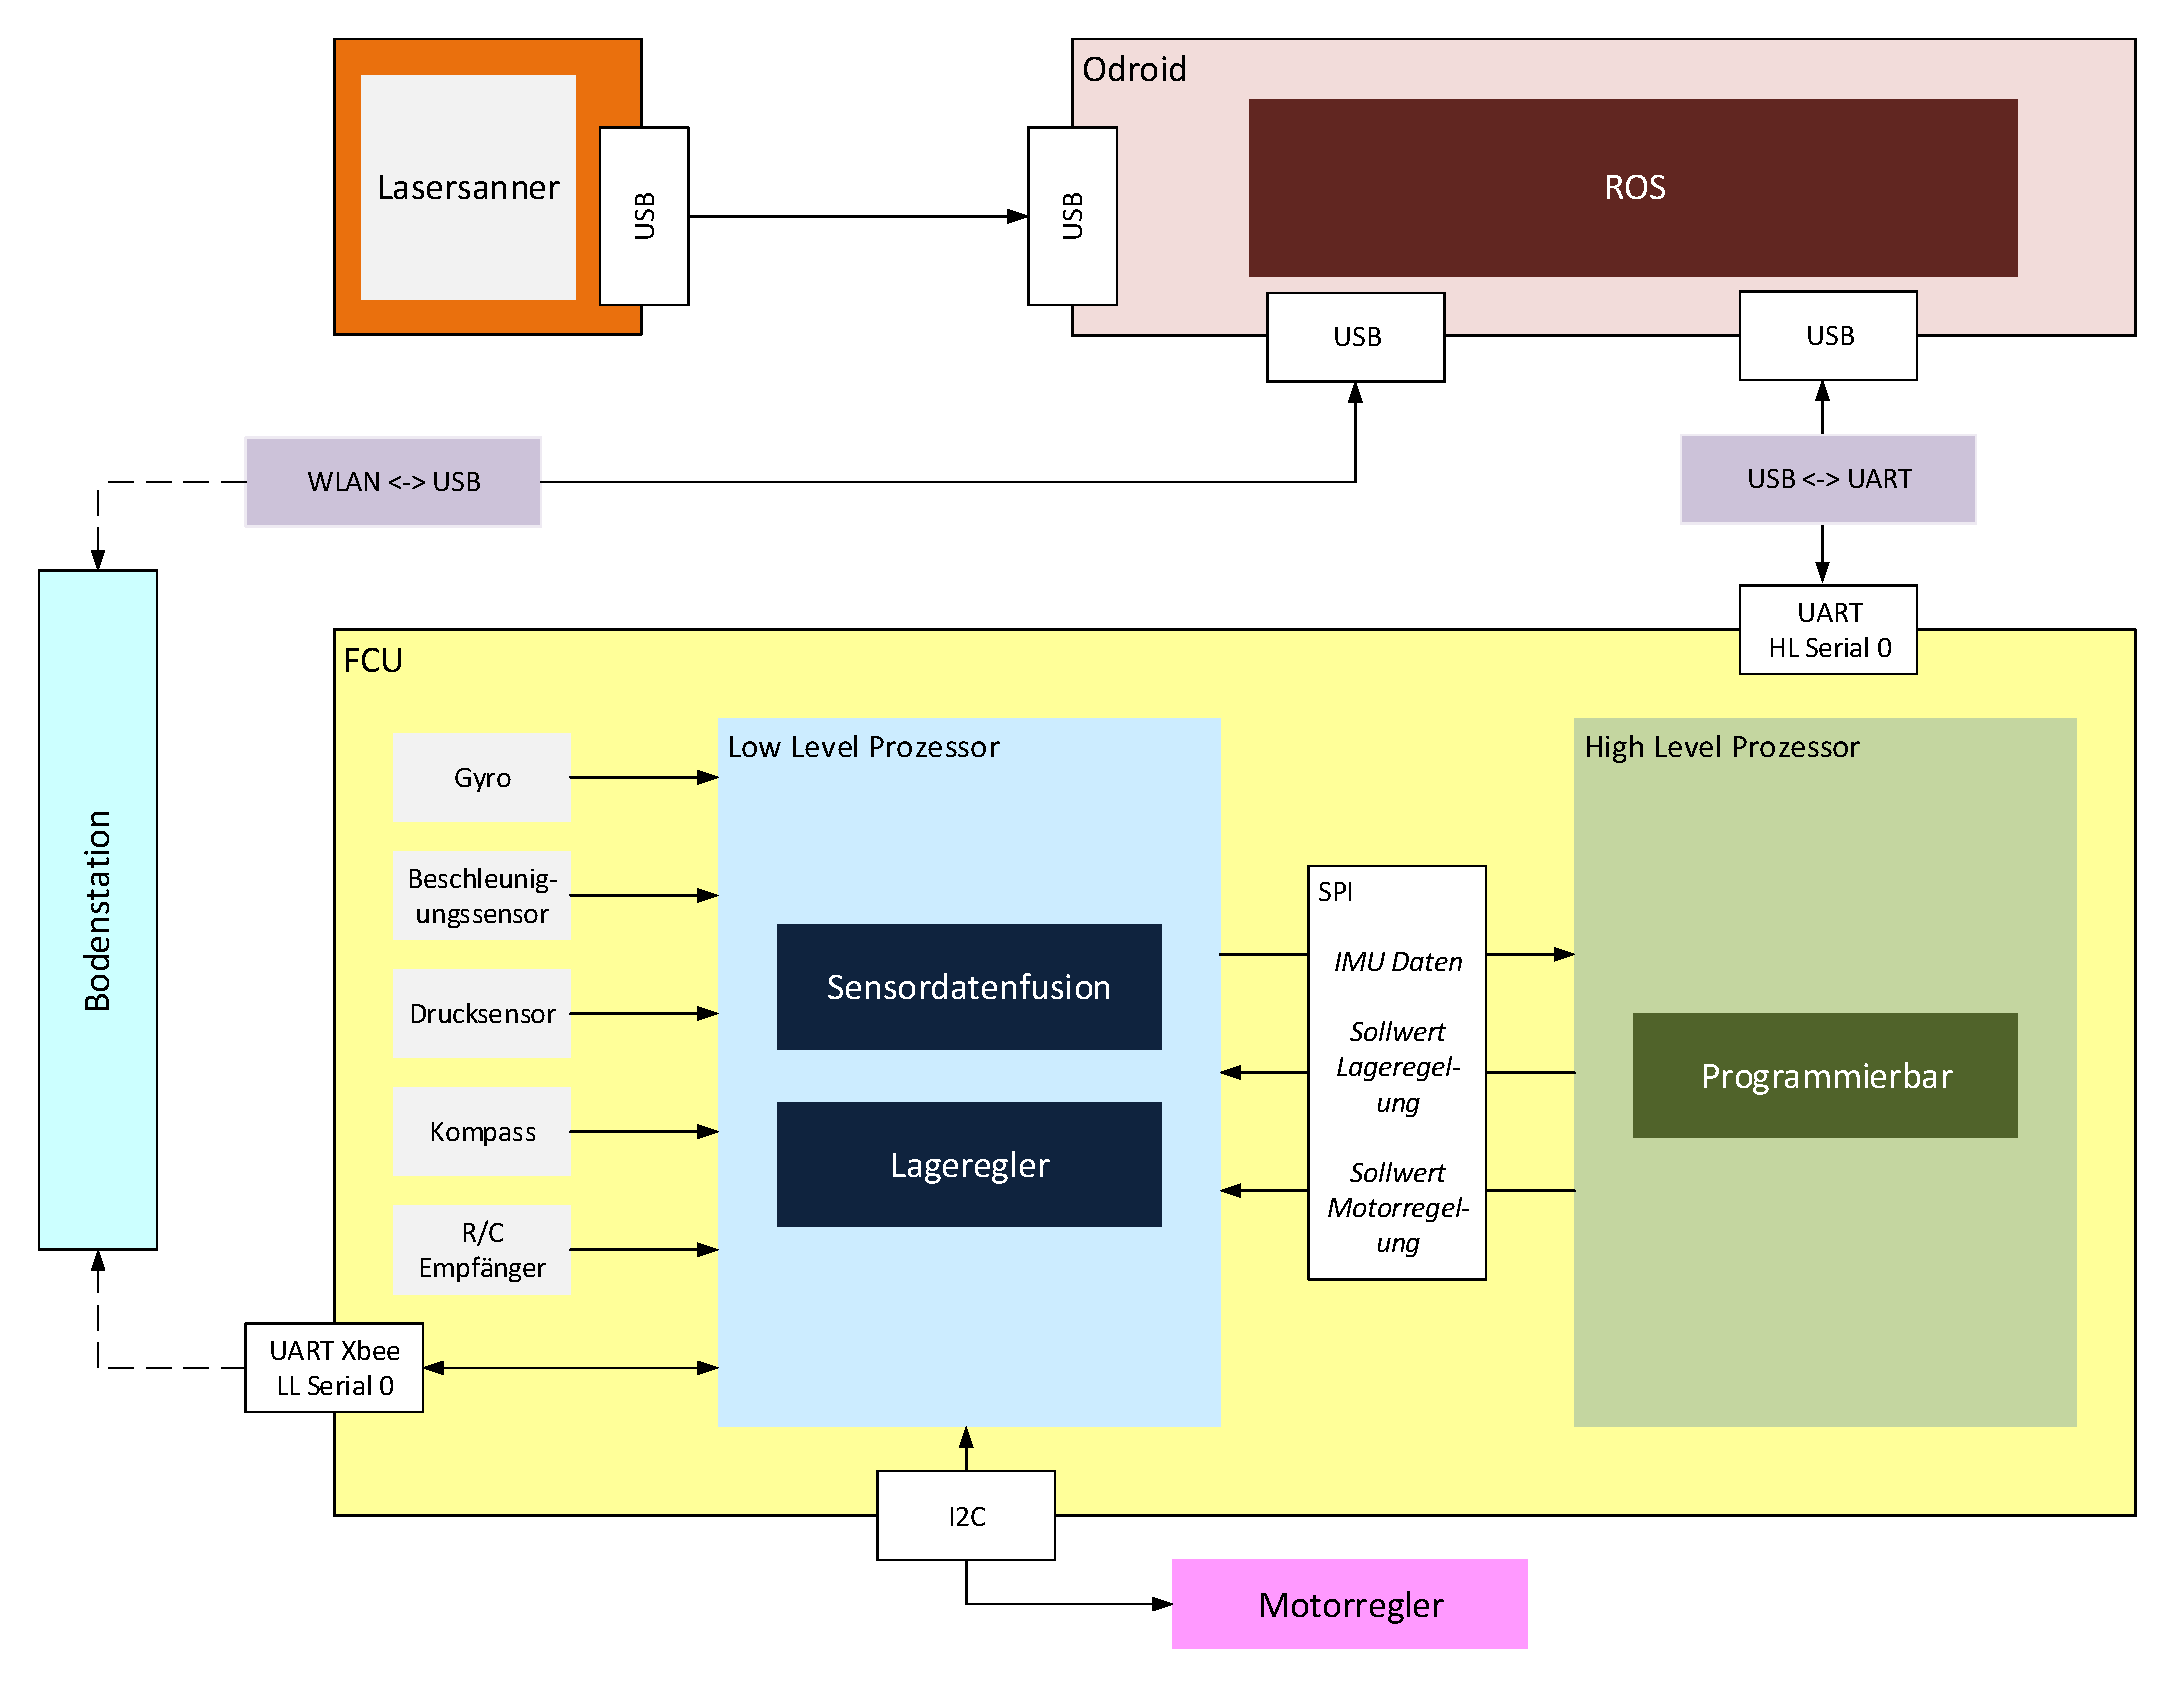
\includegraphics[width = \textwidth]{images/Kommunikationsarchitektur}
		\caption[Kommunikationsstruktur]{Kommunikationsstruktur des Quadrocopters  In Grafik fehlt das Modul zur H�henmessung Kompass auf deutsch}
		\label{fig:Kommunikationsstruktur}
\end{figure}
